\documentclass[12pt, a4paper, twoside]{scrartcl}
 %---- Allgemeine Layout Einstellungen ------------------------------------------

% Für Kopf und Fußzeilen, siehe auch KOMA-Skript Doku
\usepackage[komastyle]{scrpage2}
\pagestyle{scrheadings}
\setheadsepline{0.5pt}[\color{black}]


%Einstellungen für Figuren- und Tabellenbeschriftungen
\setkomafont{captionlabel}{\sffamily\bfseries}
\setcapindent{0em}


%---- Weitere Pakete -----------------------------------------------------------
% Die Pakete sind alle in der TeX Live Distribution enthalten. Wichtige Adressen
% www.ctan.org, www.dante.de

% Sprachunterstützung
\usepackage[ngerman]{babel}

% Benutzung von Umlauten direkt im Text
% entweder "latin1" oder "utf8"
\usepackage[utf8]{inputenc}

% Pakete mit Mathesymbolen und zur Beseitigung von Schwächen der Mathe-Umgebung
\usepackage{latexsym,exscale,stmaryrd,amssymb,amsmath}

% Weitere Symbole
\usepackage[nointegrals]{wasysym}
\usepackage{eurosym}

% Anderes Literaturverzeichnisformat
%\usepackage[square,sort&compress]{natbib}

% Für Farbe
\usepackage{color}

% Zur Graphikausgabe
%Beipiel: \includegraphics[width=\textwidth]{grafik.png}
\usepackage{graphicx}

% Text umfließt Graphiken und Tabellen
% Beispiel:
% \begin{wrapfigure}[Zeilenanzahl]{"l" oder "r"}{breite}
%   \centering
%   \includegraphics[width=...]{grafik}
%   \caption{Beschriftung} 
%   \label{fig:grafik}
% \end{wrapfigure}
\usepackage{wrapfig}

% Mehrere Abbildungen nebeneinander
% Beispiel:
% \begin{figure}[htb]
%   \centering
%   \subfigure[Beschriftung 1\label{fig:label1}]
%   {\includegraphics[width=0.49\textwidth]{grafik1}}
%   \hfill
%   \subfigure[Beschriftung 2\label{fig:label2}]
%   {\includegraphics[width=0.49\textwidth]{grafik2}}
%   \caption{Beschriftung allgemein}
%   \label{fig:label-gesamt}
% \end{figure}
\usepackage{subfigure}

% Caption neben Abbildung
% Beispiel:
% \sidecaptionvpos{figure}{"c" oder "t" oder "b"}
% \begin{SCfigure}[rel. Breite (normalerweise = 1)][hbt]
%   \centering
%   \includegraphics[width=0.5\textwidth]{grafik.png}
%   \caption{Beschreibung}
%   \label{fig:}
% \end{SCfigure}
\usepackage{sidecap}
\usepackage{float}

% Befehl für "Entspricht"-Zeichen
\newcommand{\corresponds}{\ensuremath{\mathrel{\widehat{=}}}}
\newcommand{\folgt}{\ensuremath{\mathrel{\Rightarrow}}}
\newcommand{\equals}{\ensuremath{\mathrel{\Leftrightarrow}}}
\newcommand{\degree}{\ensuremath{\mathrel{^{\circ}}}}

\newcommand{\nn}{\nonumber}
\newcommand{\tn}[1]{\textnormal{#1}}
\newcommand{\D}{\ensuremath{\mathrel{\rm d}}}

\newcommand{\const}{\tn{const}}

\newcommand{\meter}{\ensuremath{\mathrel{\tn m}}}
\newcommand{\kilogramm}{\ensuremath{\mathrel{\tn{kg}}}}
\newcommand{\second}{\ensuremath{\mathrel{\tn s}}}
\newcommand{\sekunde}{\second}

\newcommand{\volt}{\ensuremath{\mathrel{\tn V}}}
\newcommand{\pascal}{\ensuremath{\mathrel{\tn{Pa}}}}
\newcommand{\coulomb}{\ensuremath{\mathrel{\tn C}}}
\newcommand{\newton}{\ensuremath{\mathrel{\tn N}}}
\newcommand{\liter}{\ensuremath{\mathrel{\tn l}}}
\newcommand{\celsius}{\ensuremath{\mathrel{\tn C}}}
\newcommand{\fahrenheit}{\ensuremath{\mathrel{\tn F}}}
\newcommand{\joule}{\ensuremath{\mathrel{\tn J}}}
\newcommand{\kelvin}{\ensuremath{\mathrel{\tn K}}}
\newcommand{\mol}{\ensuremath{\mathrel{\tn{mol}}}}
\newcommand{\gramm}{\ensuremath{\mathrel{\tn{g}}}}

\newcommand{\kilo}{\ensuremath{\mathrel{\tn k}}}
\newcommand{\hecto}{\ensuremath{\mathrel{\tn h}}}

\newcommand{\centi}{\ensuremath{\mathrel{ \tn c}}}
\newcommand{\milli}{\ensuremath{\mathrel{ \tn m}}}
\newcommand{\micro}{\ensuremath{\mathrel{ \tn\mu }}}



%\newcommand{}{\ensuremath{\mathrel{  }}}
%\newcommand{}{\ensuremath{\mathrel{  }}}
%\newcommand{}{\ensuremath{\mathrel{  }}}


\newcommand{\person}[1]{\textsc{#1}}

 \begin{document}
 %Titelseite
\begin{titlepage}
\centering
\textsc{\Large Anfängerpraktikum der Fakultät für
  Physik,\\[1.5ex] Universität Göttingen}

\vspace*{4.2cm}

\rule{\textwidth}{1pt}\\[0.5cm]
{\huge \bfseries
  Spezifische Wärme der Luft und Gasthermometer}\\[0.5cm]
\rule{\textwidth}{1pt}

\vspace*{3.5cm}

\begin{Large}
\begin{tabular}{ll}
Praktikanten: &  Silke Andrea Teepe\\
& Marcel Kramer\\
E-Mail: & \\
Betreuer: & Alexander Schmelev\\
\end{tabular}
\end{Large}

\vspace*{0.8cm}

\begin{Large}
\fbox{
  \begin{minipage}[t][2.5cm][t]{6cm} 
    Testat:
  \end{minipage}
}
\end{Large}

\end{titlepage}
\cleardoublepage
\tableofcontents
\cleardoublepage
\setcounter{page}{1}

\section{Einleitung}
\label{sec:einleitung}

\section{Theorie}
\label{sec:theorie}
\subsection*{Zustandsänderungen}
 Die vier möglichen Abläufe für Zustandsänderungen mit jeweils einer Konstanten
\begin{itemize}
\item isotherm $T=const$
\item isochor $V=const$
\item isobar $p=const$
\item adiabatisch $\Delta Q=0$, d.h. kein Wärmeaustausch mit der Umgebung
\end{itemize}

\subsection{Die Poisson-Gleichung}
Der Adiabatenexponent $\kappa$ ist in der Poisson-Gleichung als der Quotient der spezifischen Wärmekapazitäten bei konstantem Druck und konstantem Volumen.\\
Bei einer isochore Zustandsänderung wird keine mechanische Arbeit verrichtet, es gilt also $dW = 0$, womit man für den 1. Hauptsatz der Thermodynamik 
\begin{align*}
dU &= dW + dQ \\
dU &= dQ
\end{align*}
erhält. Zieht man nun die Formel für spezifische Wärmekapazität eines Gases
\begin{align*}
c_V = \left( \frac{dQ}{dT} \right)_V
\end{align*}
hinzu, so ergibt sich 
\begin{align}
\label{eq:1}
dU = c_V \cdot dT
\end{align}\\
Für eine adiabatische Zustandsänderung gilt nun, dass kein Wärmeaustausch mit der Umgebung stattfindet, also ist $dQ = 0$ und somit gilt für den 1. Hauptsatz
\begin{align*}
dU &= dW
\end{align*}
\begin{align}
\label{eq:2}
\Rightarrow dU &= -p \cdot dV
\end{align}\\
Da die innere Energie eine Zustandsgröße ist, kann man nun \ref{eq:1} und \ref{eq:2} gleichsetzen und erhält 
\begin{align}
\label{eq:3}
c_V \cdot dT = - p \cdot dV
\end{align}\\
Geht man von einem Mol eines idealen Gas aus, so gilt $p = \frac{RT}{V}$ und durch einsetzen in \ref{eq:3} erhält man
\begin{align*}
c_V \cdot dT &= - \frac{R\cdot T}{V}\cdot dV \\
\equals c_V \cdot \frac{dT}{T} &= - R \frac{dV}{V} \\
\equals c_V \cdot ln\left(T\right) &=  - R \cdot ln\left(V\right) + C \tn{\;\;, wobei}
\end{align*}
\begin{align}
C &= \tn{Konstante} \nn\\
&= c_V \cdot ln\left(T\right) + R \cdot ln\left(V\right) \nn\\
&= ln\left(T^{c_V}V^R\right) \nn\\
\Rightarrow T^{c_V}R^V &= const   \label{eq:4}
\end{align}
Nun gilt 
\begin{align*}
c_p &= c_V + R \\
\Rightarrow R &= c_p - c_V
\end{align*}
was wenn eingesetzt in \ref{eq:4} 
\begin{align*}
T^{c_V}V^{c_p - c_V} &= const \\
\end{align*}
\begin{align}
\label{eq:5}
\Rightarrow TV^{\frac{c_p - c_V}{c_V}} &= TV^{\kappa - 1}\\
&= const \nn
\end{align}
ergibt. Setzt man nun die ideale Gasgleichung umgestellt nach T, $T = \frac{pV}{R}$, in \ref{eq:5} ein, so erhält man
\begin{align*}
TV^{\kappa -1} &= \frac{pV^{\kappa}}{R} \\
&= const
\end{align*}
Da R konstant ist, gilt also
\begin{align*}
pV^{\kappa} &= const \\
\equals p \sim V^{-\kappa}
\end{align*}

\subsection{Berechnung des Adiabatenexponenten über Freiheitsgrade}
Es gilt für die spezifischen Wärmekapazitäten bei konstantem Volumen
\begin{align*}
\frac{c_V}{R} &= \frac{f}{2} \\
\Rightarrow c_V &= \frac{f}{2}R
\end{align*}
und konstantem Druck
\begin{align*}
c_p &= c_V + R = \left( \frac{f}{2} + 1\right)R = \frac{f + 2}{2}R
\end{align*} 
Entsprechend gilt für den Adiabatenexponenten
\begin{align*}
\kappa &= \frac{c_p}{c_V} = \frac{\frac{f+2}{2}R}{\frac{f}{2}R} = \frac{f+2}{f}
\end{align*}

\subsection{Adiabatenexponent nach Rüchardt}
\begin{figure} [!h]
\centering
\label{g:1}
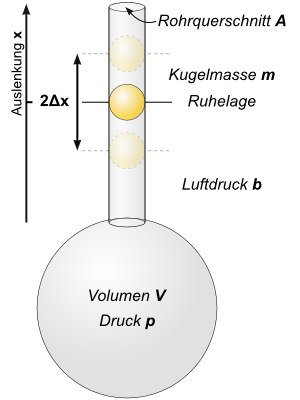
\includegraphics[scale=0.5]{Ruechardt.png}
\protect\footnotemark
\end{figure}
\footnotetext{https://lp.uni-goettingen.de/get/text/3639 Abb.4338}
Wird eine Kugel in eine Röhre geworfen wie zu sehen in Abb.\ref{g:1}, so dass kein Gas entweichen kann, führt die Kugel eine gedämpfte Schwingung aus. Grund dafür ist die periodische Umwandlung der kinetischen Energie der Kugel in einen Überdruck des Gases im Kolben und zurück.\\
Sei $m$ die Masse der Kugel, $A$ die Querschnittsfläche des Rohrs, $p$ der Gasdruck im Kolben und $b$ der Luftdruck, so gilt, wenn sich die Kugel Gleichgewicht befindet
\begin{align*}
p &= b+ \frac{mg}{A} \\
\tn{und } m\ddot{x} &= A \cdot dp
\end{align*}
wenn die Kugel um $\Delta x$ über die Gleichgewichtslage schwingt.\\
Da dieser Vorgang adiabatisch erfolgt, ist $pV^{\kappa} = const$ und man erhält mit differenzieren nach $V$
\begin{align*}
dp &= -\kappa \cdot p \frac{dV}{V} \\
&= -\kappa \frac{p \cdot A \cdot \Delta x}{V} \\
\tn{es ist also} \\
m \ddot{x} &= -\kappa \frac{p \cdot A^2 \cdot \Delta x}{V}
\end{align*}
Man erhält damit eine Schwingungsdauer $T$ von
\begin{align*}
T &= 2\pi \sqrt{\frac{m\cdot V}{\kappa \cdot A^2 \cdot p}}
\end{align*}
Mit $d$, Durchmesser des Glasrohrs ($A = \frac{1}{4} \pi d^2$) ergibt sich für den Adiabatenexponenten
\begin{align*}
\kappa &= \frac{4 \pi^2 \cdot m_{eff} \cdot V}{A^2 \cdot p \cdot T^2}
\end{align*}
$m_{eff}$ ist dabei die effektive Masse, die die Masse $m_L$ der im Rohr mitschwingenden Luftsäule beinhaltet: $m_{eff} = m + m_L$

\subsection{Der Adiabatenexponent nach Clement-Desormes}
Diese Methode beruht auf der Messung des Drucks vor und nach einer Expansion. Es wir dazu mit einem Blasebalg ein geringer Überdruck $\Delta p$ in einem Glasbehälter mit Volumen $V_0$  gegenüber dem Luftdruck $b$ erzeugt und ein thermischer Ausgleich der Kompressionswärme zu $T_0$ (Zimmertemperatur) erlaubt. Der verbleibende Überdruck wird mit dem U-Rohr Manometer gemessen (Zustand 1). \\
Nun wird durch kurzzeitiges Öffnen des Entlüftungsventils das Gas gegen den Außendruck expandiert. Die verursacht einen Verlust innerer Energie, die Temperatur des Gases sinkt (Zustand 2). Nach Druckausgleich ist wieder das Volumen $V_0$ erreicht (Zustand 3). Wärmeaustausch mit der Umgebung verursacht einen Temperaturanstieg und damit einen Anstieg des Drucks (isochor, Zustand 4) \\
Zusammenfassung der Zustände:
\begin{table}
\begin{tabular}{llll}
Zustand 1: & $V=V_0$ & $p=b+\Delta p_1$ & $T=T_0$ \\
Zustand 2: & $V=V_0+\Delta V$ & $p=b$ & $T=T_0-\Delta T$ \\
Zustand 3: & $V=V_0$ & $p=b$ & $T=T_0-\Delta T$ \\
Zustand 4: & $V=V_0$ & $p=b+\Delta p_2$ & $T=T_0$ \\
\end{tabular}
\end{table}
Der Übergang von Zustand 1 zu 2 ist adiabatisch, mit der Poisson-Gleichung erhält man
\begin{align}
\label{eq:6}
\left(b + \Delta p_1\right)V_0^{\kappa} &= b\left(V_0 + \Delta V\right)^{\kappa} \\
\label{eq:7}
\left(T_0 - \Delta T\right)\left(V_0 + \Delta V\right)^{\kappa -1} &= T_0 V_0^{\kappa -1}
\end{align}
Für $\Delta V \ll V_0$ gilt
\begin{align*}
\left(V_0 + \Delta V\right)^{\kappa} &= V_0^{\kappa}\left(1+ \frac{\Delta V}{V_0}\right)^{\kappa} \\
\sim V_0^{\kappa} + \kappa \cdot V_0^{\kappa -1}\Delta V
\end{align*}
was Umformen von \ref{eq:6} und \ref{eq:7} in 
\begin{align*}
\frac{\Delta p_1}{b} &= \kappa \frac{\Delta V}{V_0} \\
\tn{bzw.}
\frac{\Delta T}{T_0} &= \left(\kappa -1 \right) \frac{\Delta V}{V_0}
\end{align*}
ermöglicht und woraus folgt
\begin{align}
\label{eq:8}
\frac{\Delta T}{T_0} &= \frac{\kappa -1}{\kappa} \frac{\Delta p_1}{b}
\end{align}
Der Übergang von Zustand 3 zu 4 ist isochor, mit der allgemeinen Gasgleichung erhält man also
\begin{align}
\label{eq:9}
\frac{b}{b +\Delta p_2} &= \frac{T_0 -\Delta T}{T_0} \\
&= 1- \frac{\Delta T}{T_0}
\end{align}
Durch eliminieren von $\frac{\Delta T}{T_0}$ in \ref{eq:9} mittels \ref{eq:8} und auflösen nach $\kappa$ erhält man schließlich
\begin{align*}
\kappa &= \frac{\Delta p_1}{\Delta p_1 - \Delta p_2}
\end{align*} 
Für Messung der Druckdifferenzen mittels des U-Rohr Manometers werden die Höhen $h$ der Flüssigkeiten beidseitig der Spiegelskala abgelesen. Der Druck berechnet sich aus der Höhendifferenz $\Delta h = h_l - h_r$ über die Dichte der Flüssigkeit.


\section{Durchführung}
\label{sec:durchfuehrung}
\subsection{Adiabatenexponent nach Rüchardt}
Um den Adiabatenexponent mit der Methde nach \person{Rüchardt} zu bestimmen, verwendet man den linken Versuchsaufbau im Bild \ref{fig:aufbau}.
Für jedes der zu untersuchenden Gase Luft, Kohlenstoffdioxid und Argon ist dafür zu sorgen, dass der Glaskolben ausschließlich mit diesem Gas gefüllt ist.
Für CO$_2$ und Argon bedeutet das, das Regulierungsventil und das Entlüftungsventil für ca. 3 min zu öffnen damit das Gas ausgetauscht wird.
Nun muss der Gasdruck mittels Regulierungsventil so eingestellt werden, dass der Schwingkörper symmetrisch um die Austrittsöffnung schwingt ohne an eines der enden des Glasrohrs zu stoßen.\\
Nach der Einstellung der Schwigung kann die Messung beginnen. Es soll 10mal die Zeit für eine Periode und je 3mal die Zeit für 10, 20, 50 und 100 Perioden gemessen werden.
Die Zeiten sind zu messn, indem man die zu messende Anzahl Perioden am Zähler der Lichtschranke einstellt und dan den Startknopf drückt.\\
Neben den Zeiten sind noch der Umgebungsluftdruck, die Masse des Schwingkörpers, das Volumen des Glaskolben und den Durchmesser des Glasrohrs zu bestimmen.
\subsection{Adiabatenexponent nach Clement-Desormes}
Um den Adiabatenexponent mit der Methde nach \person{Clement-Desormes} zu bestimmen, verwendet man den rechten Versuchsaufbau im Bild \ref{fig:aufbau}.
Mit dem Blasebalg ist der Druck in dem Glasbehälter zu erhöhen und dann mit dem Verschlussventil zu verschließen.
Nun warte man den Temperaturausgleich mit der Umgebung ab und sobald sich die Manometerspiegel nicht mehr verändert ist die Druckdifferenz $\Delta p_1$ bzw. die Flüssikeitssäulenhöhe $\Delta h_1$ zu notieren.
Daraufhin ist das Entlüftungsventil kurzzeitig zu öffnen und nach erneutem Temperaturausgleich die neue Flüssikeitssäulenhöhe $\Delta h_2$ zu bestimmen.\\
Dieser Versuch ist mehrmals für 3 verschiedene Öffnungszeiten des Entlüftungsventil zu wiederholen. Die empfohlenen Zeiten sind ca. $0.1\sekunde$, $1\sekunde$ und $5\sekunde$.

\begin{figure}[!h]
 \centering
 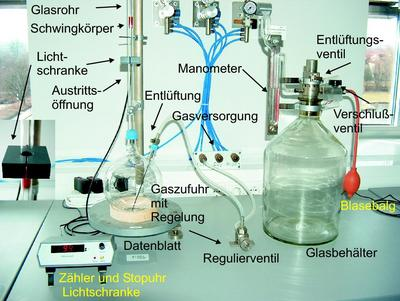
\includegraphics[scale=1.0]{aufbau.png}
 \caption{\label{fig:aufbau}Versuchsaufbau\protect\footnotemark}
\end{figure}
\footnotetext{https://lp.uni-goettingen.de/get/text/3639  Abb.3725}

\section{Auswertung}
\label{sec:auswertung}

\subsection{Rüchardt}
Vor dem Versuch wurde der Umgebungsdruck im Raum gemessen. Dieser betrug $p_0=1004,1\hecto\pascal$. Außerdem wurden folgende Werte von dem Versuchsaufbau abgelesen: $M=4,88\gramm$ (Masse des schwingenden Körpers), $d=9,97\milli\meter$ (Rohrdurchmesser) und $V=2300\centi\meter^3$ (Kolbenvolumen). Der Fehler des Umgebungsdrucks ist klein und kann daher vernachlässigt werden. Die abgelesenen Wert waren ohne Fehlerangabe und werden daher als exakt angenommen.\\

Aus diesen Werten berechnet sich der Druck im Kolben mit Formel \ref{eq:1} und $A=\pi\cdot (d/2)^2$ zu $p=101024\pascal$. Um die effektive Masse des schwingenden Körpers zu bestimmen muss die Masse der mitschwingenden Luftsäule $m_L=hA\rho_L$ beachtet werden. Dabei ist $\rho_L=1,225\kilogramm/\meter^3$ die Luftdichte bei $15\degree\celsius$ und $h=11,5\centi\meter$ die Höhe der Luftsäule. Die effektive Masse ist dann
\begin{align*}
m_{eff}=m+m_L=4,89\cdot10^-3\kilogramm.
\end{align*}
Nun kann aus denn Messwerten und der Formel
\begin{align*}
\kappa=\frac{c_p}{c_V}=\frac{64\cdot m_{eff}\cdot V}{T^2\cdot p\cdot d^4}
\end{align*}
für jede Messung der Adiabatenexponent bestimmt werden. Die gewichteten Mittelwerte der Ergebnisse sind in Tabelle \ref{tab:ruechardt} zusammen mit dem Fehler aufgeführt. Zur Fehlerberchnung wurde davon ausgegangen, dass die Stopuhr mit einem systematischen Fehler $\sigma_T$ von maximal 3\% behaftet ist. Der Gesamtfehler ergibt sich dann durch Fehlerfortpflanzung zu
\begin{align*}
\sigma_\kappa=\sqrt{\left(\frac{\partial\kappa}{\partial T}\right)^2\sigma_T^2}=\sqrt{\left(\frac{2\cdot64\cdot m\cdot V}{T^3\cdot p \cdot d^4}\right)^2\sigma_T^2}.
\end{align*}

\begin{table} [H]
\centering
\begin{tabular}{|r|c|c|c|c|} \hline
    Gas & $\kappa$ & $\sigma_\kappa$ & $f$ & $\sigma_f$ \\ \hline
    Luft & 1,28& 0,02 & 7,14 &  0,14\\
    $\rm{CO_2}$ & 1,22& 0,02 & 9,09 & 0,18 \\
    Arg & 1,53& 0,02 & 3,77 &  0,08 \\ \hline
 \end{tabular} 
 \caption{\label{tab:ruechardt}Ergebnisse nach Rüchardt}
\end{table}

Zum Schluss lassen sich die Freiheitsgrade mit Formel \ref{eq:2} berechnen
\begin{align*}
f=\frac{2}{\kappa-1}
\end{align*}
mit dem Fehler
\begin{align*}
\sigma_f=\sqrt{\left(\frac{\partial f}{\partial \kappa}\right)^2\sigma_\kappa^2}=\frac{2}{\left(k-1\right)^2}\sigma_\kappa.
\end{align*}
Die Ergebnisse sind ebenfalls in Tabelle \ref{tab:ruechardt} zu finden.




\subsection{Clement-Desormes}

Die Adiabatenexponente nach Clement-Desormes berechnte sich durch
\begin{align*}
\kappa=\frac{c_p}{c_V}=\frac{\Delta h_1}{\Delta h_1-\Delta h_2}
\end{align*}
mit dem Fehler
\begin{align*}
\sigma_\kappa=\sqrt{\left(\frac{\partial\kappa}{\partial h_1}\right)^2\sigma_{\Delta h_1}^2+\left(\frac{\partial\kappa}{\partial h_2}\right)^2\sigma_{\Delta h_2}^2}=\sqrt{\frac{\Delta h_2}{(\Delta h_2-\Delta h_1)^2}\sigma_{\Delta h_1}+\frac{\Delta h_1}{(\Delta h_1-\Delta h_2)^2}\sigma_{\Delta h_2}}
\end{align*}
Die berechneten gewichteten Mittelwerte für die einzelnen Zeitintervalle sind in Tabelle \ref{tab:clement} aufgeführt. Der Ablesefehler wurde mit $\sigma_{\Delta h_1}=\sigma_{\Delta h_2}=1\milli\meter$ abgeschätzt. Insgesamt beträgt der gewichtete Mittelwert aus den Messdaten
\begin{align*}
\kappa=1,35\pm0,01.
\end{align*}

\begin{table} [H]
\centering
\begin{tabular}{|r|c|c|} \hline
    $T\,[s]$ & $\kappa$ & $\sigma_\kappa$ \\ \hline
    $0,1$ & 1,38& 0,03 \\
    $1,0$ & 1,38& 0,03\\
    $5,0$ & 1,3& 0,03\\ \hline
 \end{tabular} 
 \caption{\label{tab:clement}}
\end{table}
Nun soll noch der gewichtet Mittelwert von $\kappa$ für Luft aus den beiden Experimenten gebildet werden. Dieser berechnet sich zu
\begin{align*}
\kappa=\frac{\kappa_R/\sigma_{\kappa_R}^2+\kappa_C/\sigma_{\kappa_C}^2}{1/\sigma_{\kappa_R}^2+1/\sigma_{\kappa_C}^2}\pm\sqrt{\left(\frac{1}{\sigma_{\kappa_R}^2}+\frac{1}{\sigma_{\kappa_C}^2}\right)^{-1}}=1,34\pm0,02
\end{align*}


\section{Diskussion}
\label{sec:diskussion}
Der theoretische Wert des Adiabatenexpnenten von Luft liegt bei $\kappa=1,40$. Unser Ergebnis liegt zwar nicht in der Fehlertoleranz, weicht aber nur um weniger als 5\% von diesem Wert ab. Bei der Berechnung nach Rüchardt fällt auf, dass die Werte des Adiabatenexpnenten für alle drei Gase deutlich unter dem theoretisch zu erwartenden Werten liegen. Daher liegt die Vermutung nahe, dass hir ein systematischer Fehler vorliegt. Dieser Fehler setzt sich in der Berechnung der Freiheitsgrade fort, was deren Abweichungen erklärt. 



\newpage
\section*{Anhang}

\begin{table} [H]
\centering
\begin{tabular}{|c|c||c|c|c|} \hline
    Messung & Perioden & Luft & CO$_2$ & Ar \\\hline
    $1 $&$ 1 $&$ 751 $&$ 768 $&$ 685$ \\
    $2 $&$ 1 $&$ 750 $&$ 769 $&$ 687$ \\
    $3 $&$ 1 $&$ 749 $&$ 770 $&$ 686$ \\
    $4 $&$ 1 $&$ 751 $&$ 769 $&$ 687$ \\
    $5 $&$ 1 $&$ 749 $&$ 771 $&$ 687$ \\
    $6 $&$ 1 $&$ 749 $&$ 770 $&$ 687$ \\
    $7 $&$ 1 $&$ 751 $&$ 771 $&$ 685$ \\
    $8 $&$ 1 $&$ 751 $&$ 770 $&$ 686$ \\
    $9 $&$ 1 $&$ 749 $&$ 771 $&$ 686$ \\
    $10 $&$ 1 $&$ 750 $&$ 768 $&$ 686$ \\
    \hline
    $1 $&$ 10 $&$ 7512 $&$ 7698 $&$ 6862$ \\
    $2 $&$ 10 $&$ 7520 $&$ 7702 $&$ 6864$ \\
    $3 $&$ 10 $&$ 7524 $&$ 7701 $&$ 6866$ \\
    \hline
    $1 $&$ 20 $&$ 15012 $&$ 15407 $&$ 13735$ \\
    $2 $&$ 20 $&$ 15007 $&$ 15412 $&$ 13737$ \\
    $3 $&$ 20 $&$ 15028 $&$ 15419 $&$ 13734$ \\
    \hline
    $1 $&$ 50 $&$ 37540 $&$ 38542 $&$ 34350$ \\
    $2 $&$ 50 $&$ 37560 $&$ 38533 $&$ 34345 $\\
    $3 $&$ 50 $&$ 37567 $&$ 38573 $&$ 34352 $\\
    \hline
    $1 $&$ 100 $&$ 75176 $&$ 77110 $&$ 68726$ \\
    $2 $&$ 100 $&$ 75192 $&$ 77138 $&$ 68722$ \\
    $3 $&$ 100 $&$ 75216 $&$ 77157 $&$ 68544$ \\
    \hline
 \end{tabular} 
 \caption{\label{tab:}Messwerte in Millisekunden für den Versuch nach Rüchardt}
\end{table}


\begin{table} [H]
\centering
\begin{tabular}{|c|c|c|} \hline
    Öffnungszeit & $\Delta h_1$ [\milli\meter] & $\Delta h_2$ [\milli\meter]  \\			\hline
	$0,1$ & $48$ & $14$ \\
	$0,1$ & $32$ & $8$\\
	$0,1$ & $31$ & $10$\\
    \hline
	$1,0$ & $54$ & $14$\\
	$1,0$ & $40$ & $10$\\
	$1,0$ & $35$ & $11$\\
    \hline
	$5,0$ & $44$ & $12$\\
	$5,0$ & $32$ & $7$\\
	$5,0$ & $37$ & $7$\\
    \hline
 \end{tabular} 
 \caption{\label{tab:}Messwerte für den Versuch nach Clement-Desormes}
\end{table}





%\begin{wraptable}{r}{5cm}
%\centering
%\begin{tabular}{r|l}
% \end{tabular} 
% \caption{\label{tab:}}
%\end{wraptable}

%\begin{table}
%\centering
%\begin{tabular}{r|c}
%    
% \end{tabular} 
% \caption{\label{tab:}}
%\end{table}




\end{document}
